\chapter[Solução]{solução}
  Este capítulo tem como objetivo discutir a solução utilizada durante o
desenvolvimento, assim como os resultados obtidos durante a realização do mesmo. Dentre estes
resultados, estão presentes as fontes de erros levantadas com a experiência do desenvolvimento,
suas respectivas correções, dentro do possível, e a análise da viabilidade da utilização do
sistema no contexto da reabilitação motora. Desse modo, este
capítulo está dividido nas seções: \ref{sol:solucao}, \ref{sol:fontesErro} e \ref{sol:viabilidade}.

\section{Solução}\label{sol:solucao}
  Nesta seção serão apresentadas as features envolvidas na solução do sistema,
além das ferramentas usadas. Esta será dividida em Arquitetura (\ref{sub:arquitetura}), Funcionalidades-\textit{features}(\ref{sub:solFeatures}) e
ferramentas(\ref{sub:solFerramentas}).

\subsection{Arquitetura}\label{sub:arquitetura}
  Dentro do Unity 3d não há uma arquitetura específica, isso fica a cargo dos desenvolvedores. Porém podemos dividir o trabalho no unity em duas partes,
a primeira é a parte de vizualização, onde ele desponibiliza um espaço 3d para a inserção dos \textit{gameObjects} e criação das cenas. Um projeto pode
ter mais de uma cena e uma cena pode conter vários \textit{gameObjects}. A segunda é com os chamados \textit{scripts}, que são os códigos que podem
ser adicionados em um \textit{gameObject} dando-lhe a lógica de como se deve comportar durante uma cena de um projeto. Esses códigos podem ser escritos
nas linguagens \textit{javascript} e em C\#.

  Para o desenvolvimento do sistema, podemos ver o diagrama de classe \ref{diagramaClasse}.

  A arquitetura dos scripts ficou um pouco focada na classe \textit{KinectManager} pois ela é a responsável pela comunicação com o kinect.
Abaixo falaremos um pouco sobre o papel de cada classe:

\begin{itemize}
  \item \textit{\textbf{KinectManage}} : Classe responsável pela comunicação com o kinect;
  \item \textit{\textbf{GetCsv}} : Classe responsável por fazer o parser do arquivo csv do movimento desejado;
  \item \textit{\textbf{AvatarController}} : Classe responsável por passar o movimento do usuário para o avatar;
  \item \textit{\textbf{StoredMovimentAvatarController}} : Classe responsável por movimentar o avatar de acordo com o movimento parseado;
  \item \textit{\textbf{GetJointPosition}} : Classe responsável por escrever as posições de todas as juntas e exportar para csv;
  \item \textit{\textbf{KinectGesture}} : Classe com alguns gestos;
  \item \textit{\textbf{KinectWrapper}} : Classe que detém as várias estruturas e importações dll;
  \item \textit{\textbf{KinectManage}} : Classe responsável por guardar as informações dos movimentos parseado;
\end{itemize}


  \begin{figure}[!h]
  \centering
  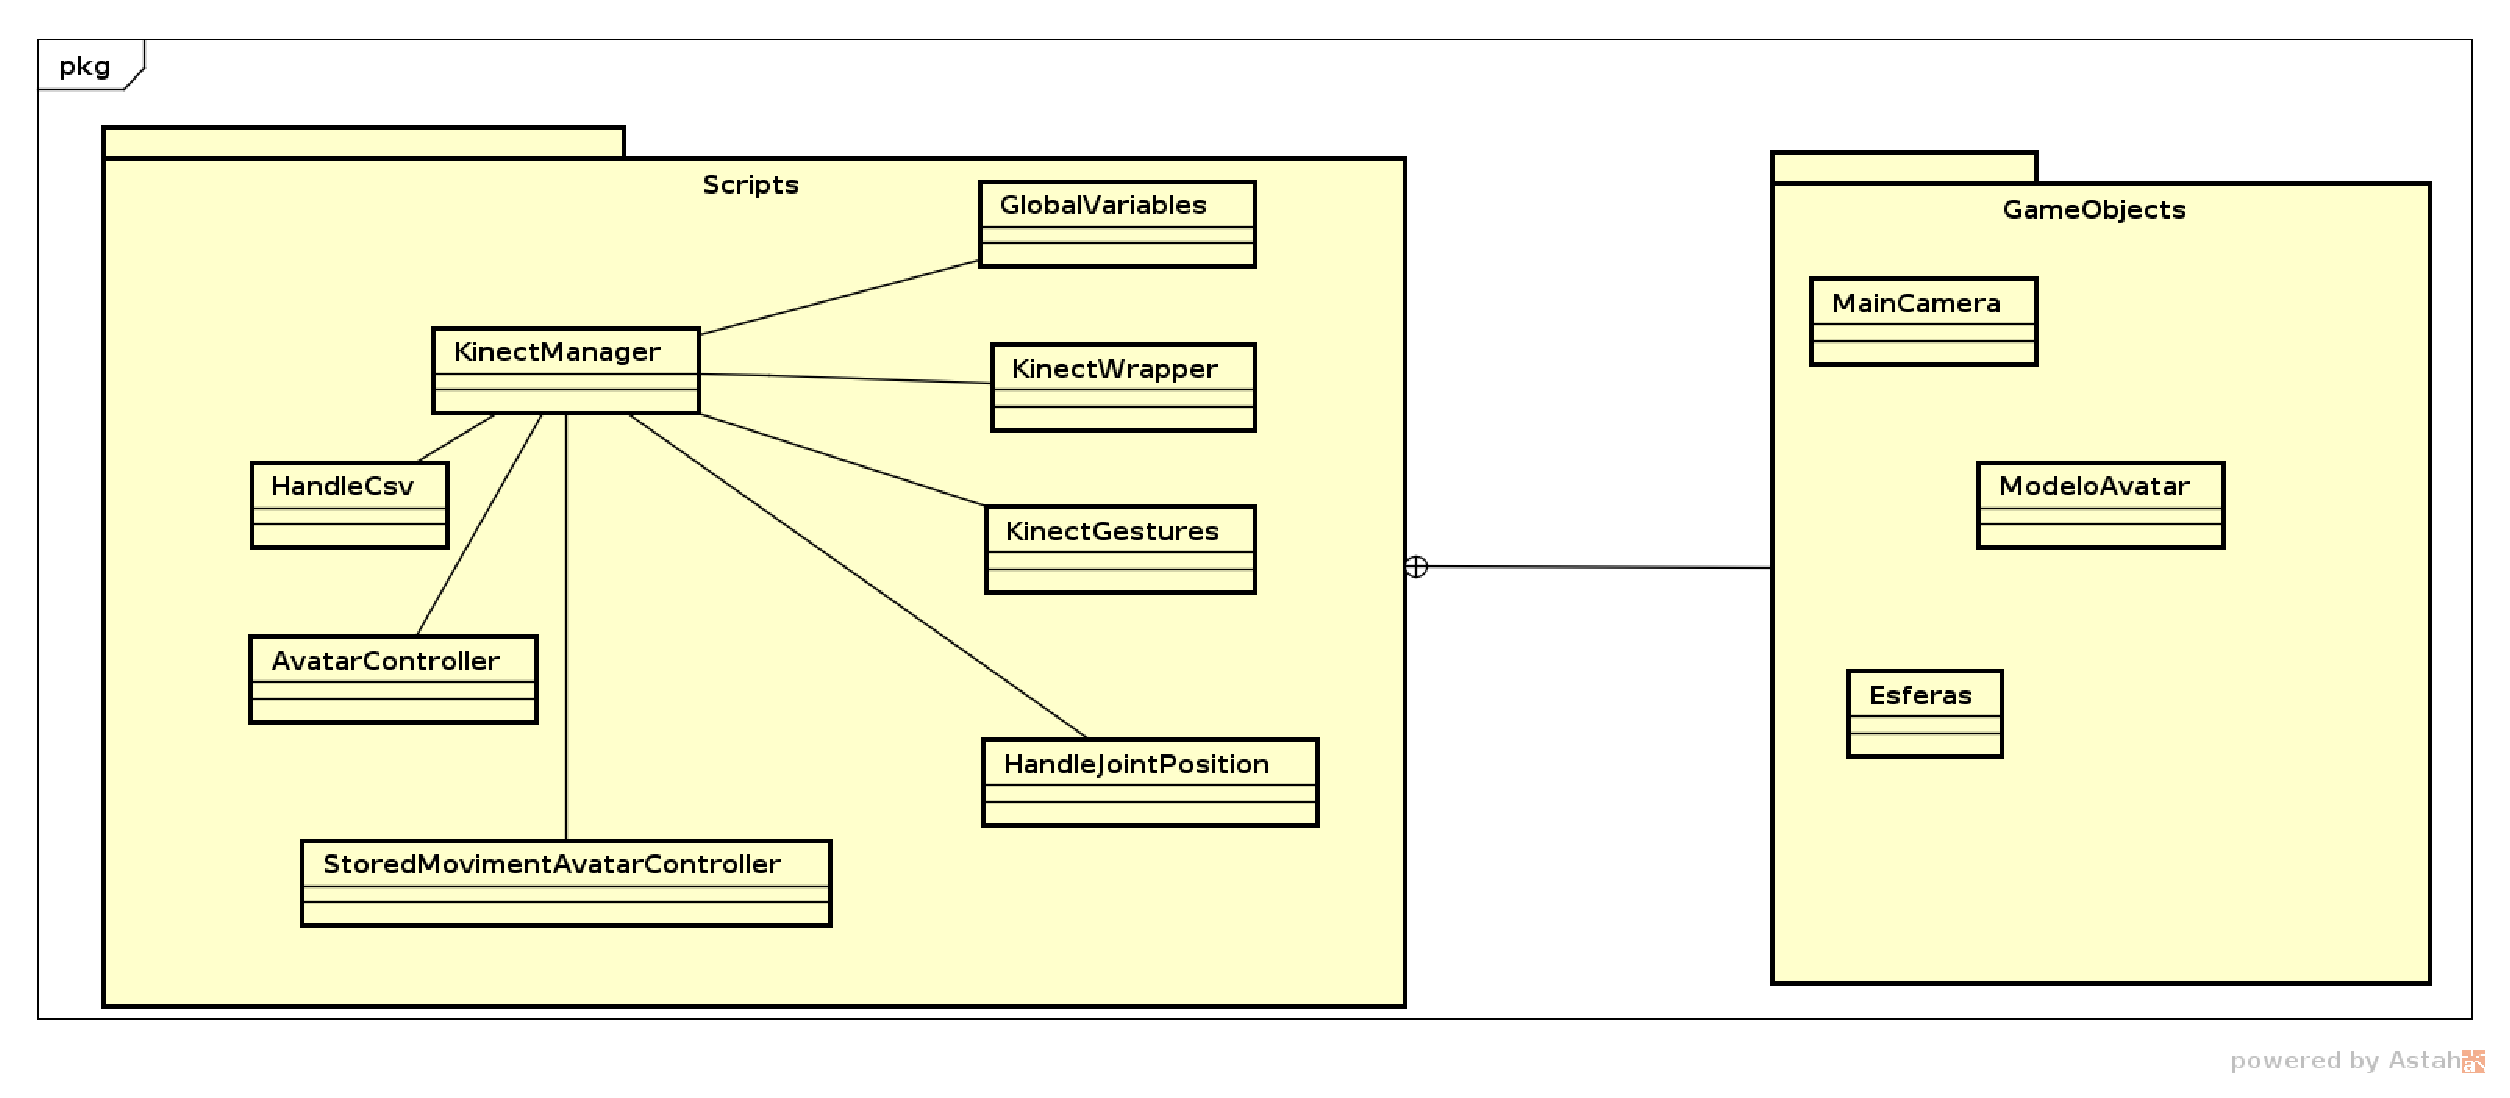
\includegraphics [keepaspectratio=true,scale=0.45]{figuras/DiagramaDeClasse.eps}

  \caption{Diagrama de classe referente ao sistema}
  \label{diagramaClasse}
  \end{figure}


\subsection{Funcionalidades - \textit{features}}\label{sub:solFeatures}
  As \textit{features} no desenvolvimento ágil é um pedaço de funcionalidade que oferece valor comercial \cite{versionOne}.
Geralmente as \textit{features} tem uma granularidade maior que as \textit{User Stories}(Histórias de usuário~\ref{historias}).
Podemos dizer que algumas features são compostas de \textit{User Stories}.

  O sistema possui três features, gravação de movimento, leitura de arquivo do movimento desejado e análise da repetição do movimento:
\begin{enumerate}
  \item \textbf{Gravar movimento:} Essa funcionalidade permite a gravação do movimento, deve ser feito pelo profissional fisioterapeuta
  para uma correta execução. Será esse movimento que o sistema usará como gabarito. O sistema retorna um arquivo csv.
  \item \textbf{Ler arquivo de movimento:} Essa funcionalidade espera um arquivo csv e armazena o movimento no sistema.
  \item \textbf{Praticar movimento:} Essa funcionalidade mostra a correta execução do movimento e analisa com o movimento do paciente.
\end{enumerate}

\subsection{Ferramentas}\label{sub:solFerramentas}
  Para o desenvolvimento do sistema foram usadas diversas ferramentas, a seguir serão apresentadas junto
dos artefatos gerados.

\subsection{Código}\label{sub:codigo}
  Para a edição e criação do código foi usado o Micorosoft Visual Studio que é uma IDE\textit{(Integrated development enviroment)} disponibilizada pela microsoft, podendo ser
encontrada \href{https://www.visualstudio.com/pt-br/?rr=https%3A%2F%2Fwww.google.com.br%2F}{aqui} gratuitamente.

\subsection{Diagrama de sequência}\label{sub:diagramaSequencia}
  Consiste em um diagrama que tem o objetivo de mostrar como as mensagens entre os objetos são trocadas no decorrer do tempo para a realização de uma operação.\cite{diagramaSequencia}
Como pode ser visto em \ref{diagramaFisio} e \ref{diagramaPaciente}, existe dois momentos de trocas de mensagens, uma com o usuário como fisioterapeuta e outra
com o paciente.

\begin{figure}[!h]
\centering
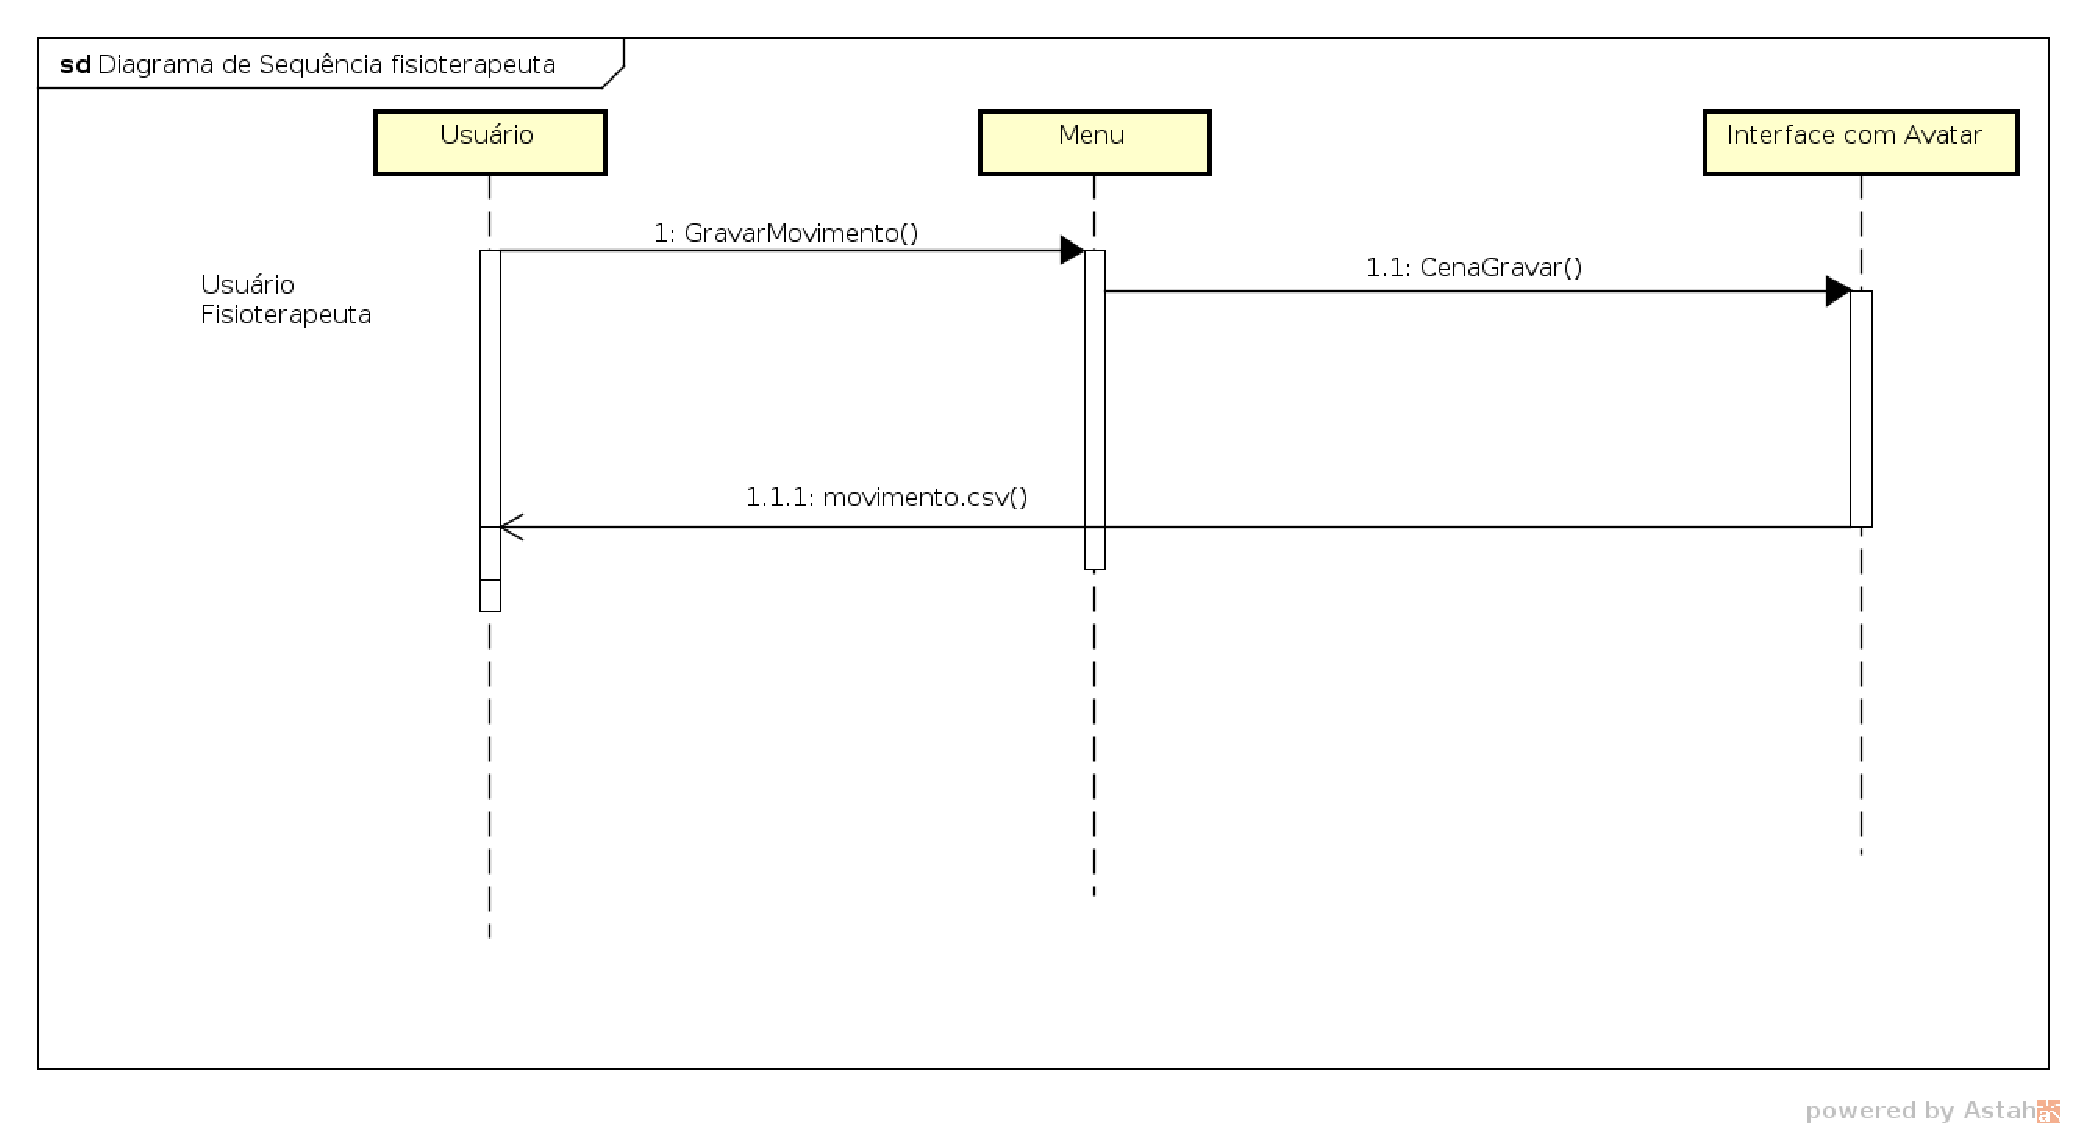
\includegraphics [keepaspectratio=true,scale=0.45]{figuras/diagramaFisio.eps}

\caption{Diagrama de sequência referente ao uso do fisioterapeuta}
\label{diagramaFisio}
\end{figure}


\begin{figure}[!h]
\centering
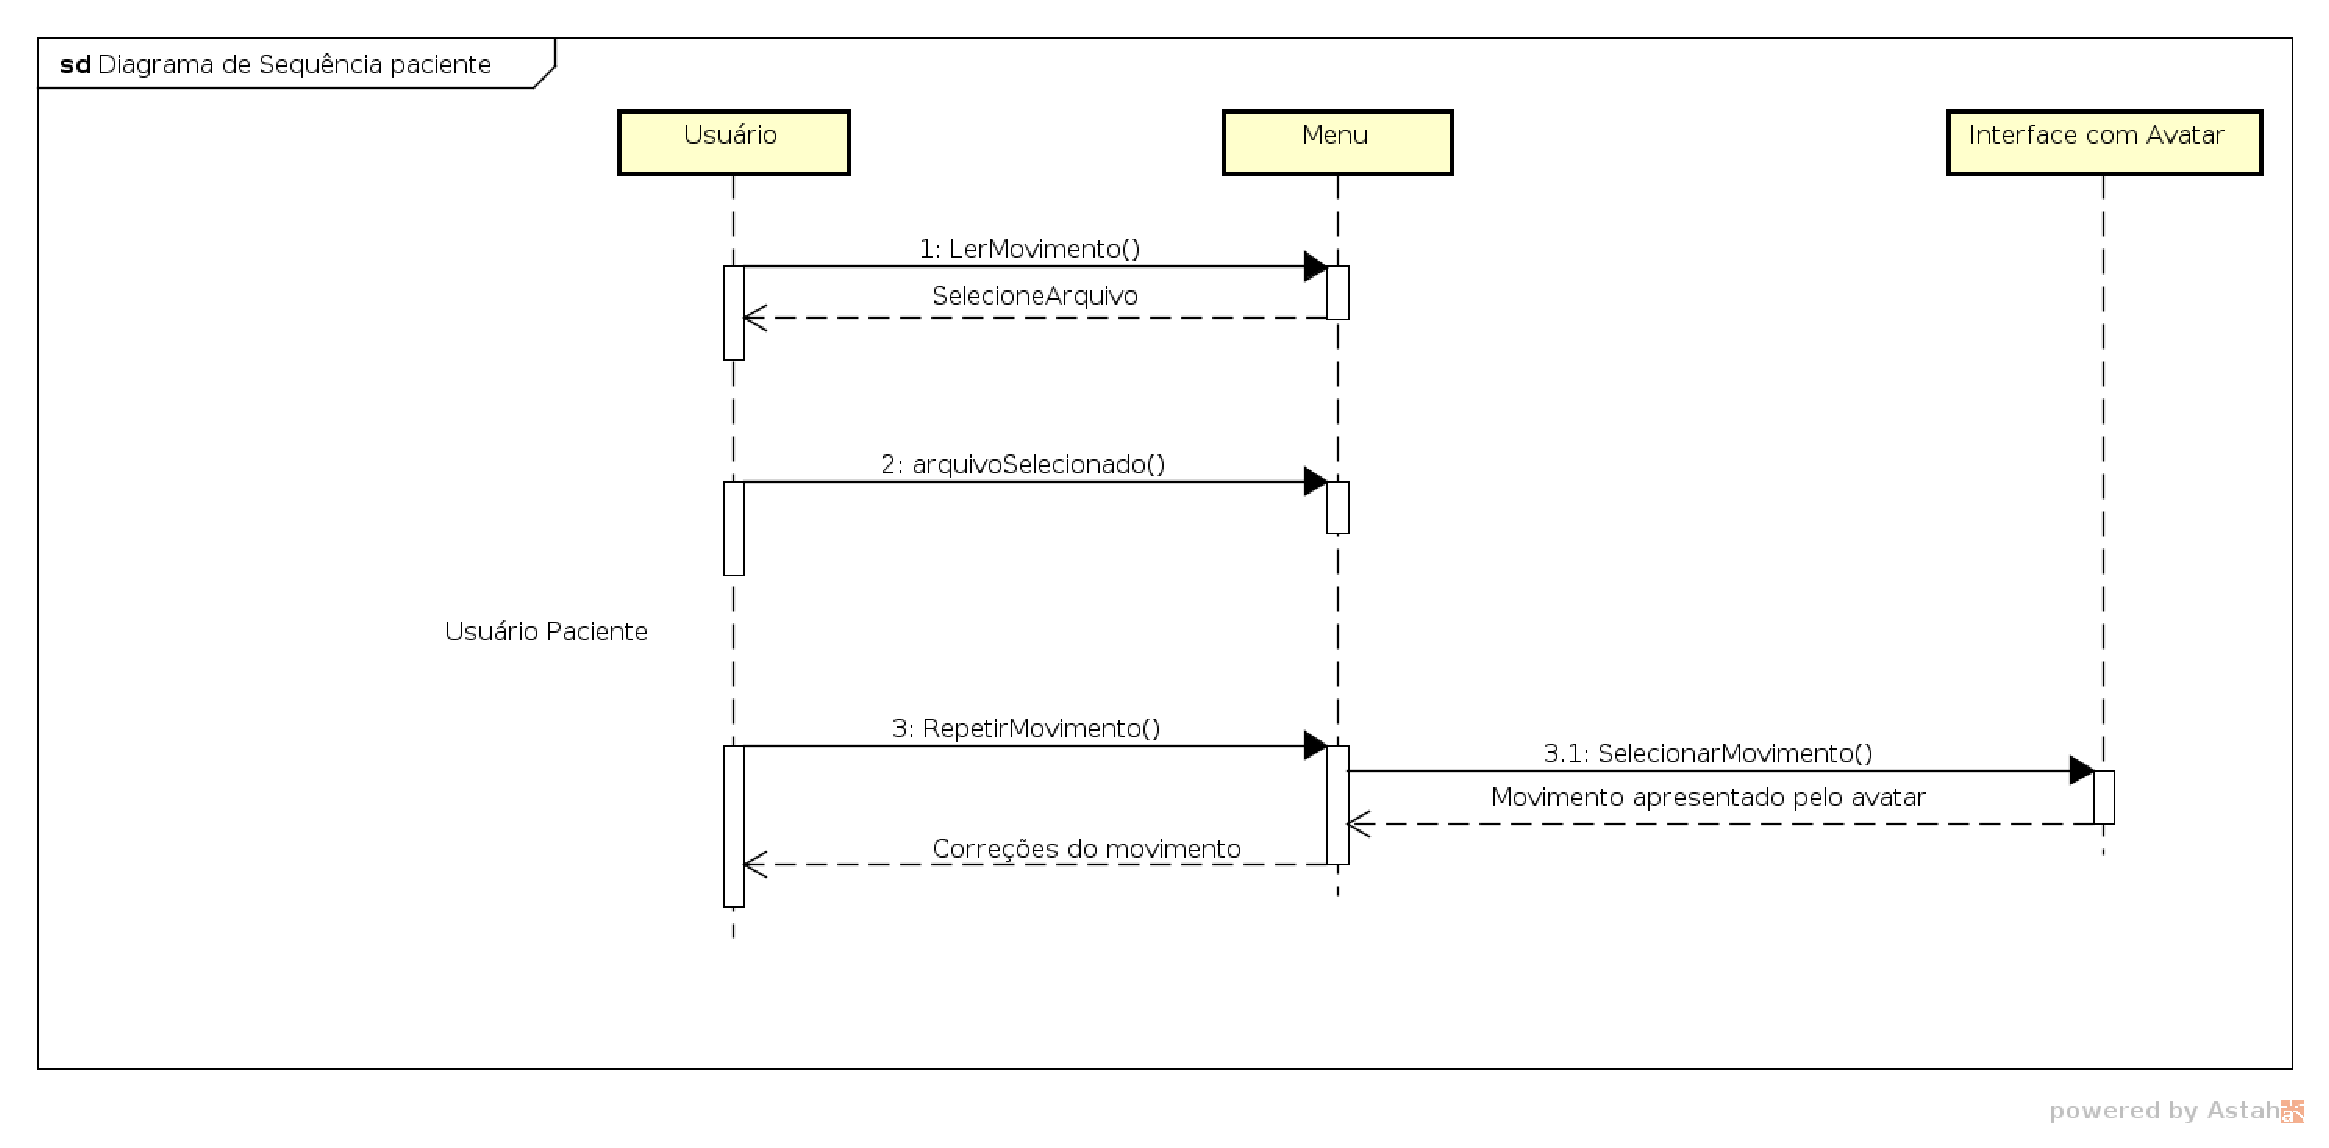
\includegraphics [keepaspectratio=true,scale=0.45]{figuras/diagramaPaciente.eps}

\caption{Diagrama de sequência referente ao uso do paciente}
\label{diagramaPaciente}
\end{figure}

  Para a criação desses artefatos foi utilizado a ferramenta Astah community que pode ser encontrada \href{http://astah.net/download#community}{aqui} gratuitamente.


\subsection{\textit{Kanban}}\label{sub:kanban}
  \textit{Kanban} é um termo de origem japonesa e significa literalmente “cartão” ou “sinalização”.
Este é um conceito relacionado com a utilização de cartões (post-it e outros) para indicar o andamento dos fluxos de produção em empresas de fabricação em série.\ref{kanban}

  Ao longo do desenvolvimento foi utilizado o \textit{trello}  que é uma espécie de \textit{kanban online}, ele pode ser acessado \href{https://trello.com/}{aqui} gratuitamente.

\section{Fontes de Erro}\label{sol:fontesErro}
\section{Análise de viabilidade}\label{sol:viabilidade}
